\section{A model-checker for process models\label{section:tool-model-checker}}

Our model-checker for guarded hMSC extends the compositional model-checking technique presented in \cite{Giannakopoulou:2003}. The latter allows model-checking LTS state machines against FLTL safety properties. Our model-checker extends this so as to take a g-hMSC or a g-LTS an input. 

The model-checking technique is illustrated on Fig.~\ref{image:model-checking-technique}. Let us read it backwards:
\begin{itemize}
\item Roughly, compositional model-checking consists in searching for an accepting state in the composition of two automata: a LTS for the model (top), the other for the negation of a safety property (the tester automaton at bottom).
\item The LTS model is synthesized from the g-hMSC and fluent definitions using the techniques described in Chapter \ref{chapter:deductive}.
\item The tester automaton is synthesized using the technique described in \cite{Giannakopoulou:2003}. Roughly, it consists in composing a B\"uchi automaton for the negation of the safety property with fluent automata and a synchronizer. 
\end{itemize} 

\begin{figure}
\centering\scalebox{.525}{
  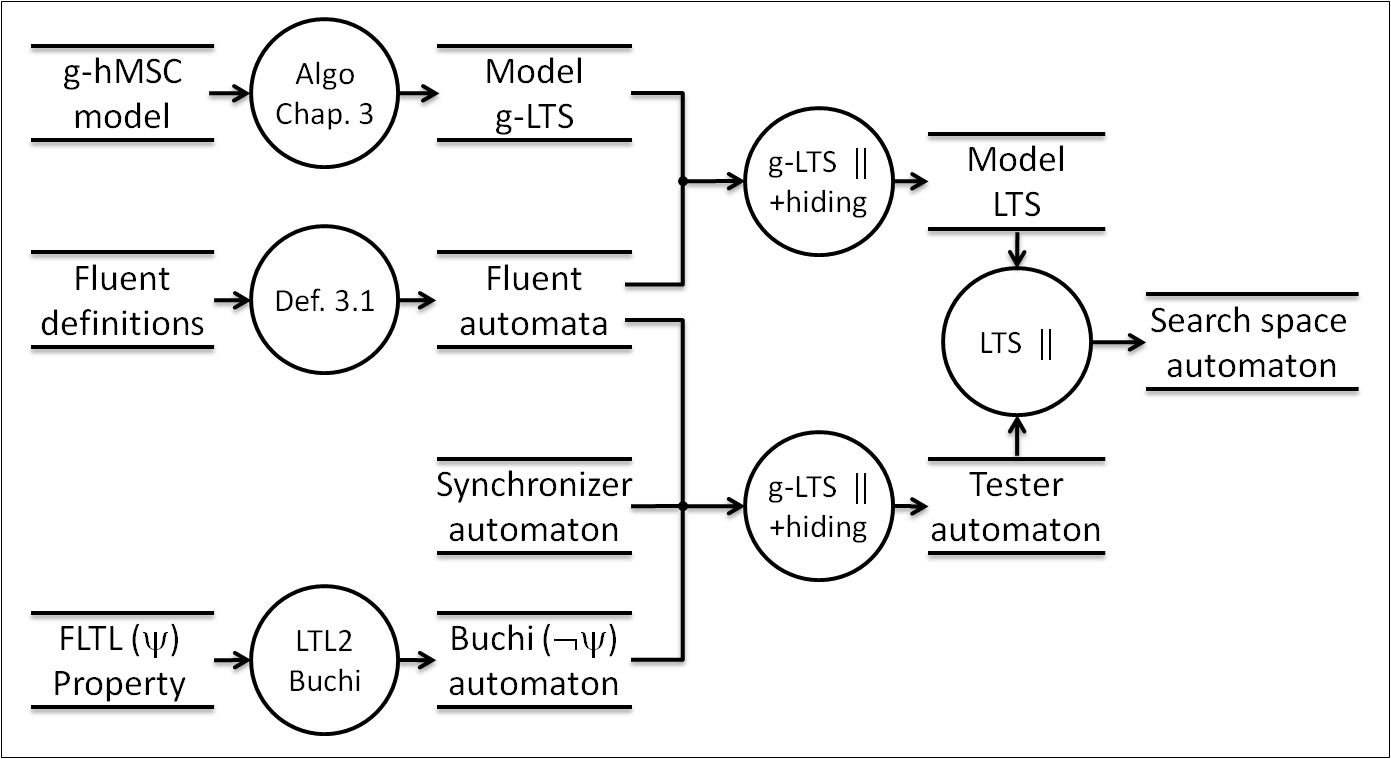
\includegraphics[trim=3mm 3mm 3mm 3mm, clip]{src/7-tool-support/images/model-checking-technique}}
  \caption{Model-checking guarded hMSC: automaton compositions\label{image:model-checking-technique}}
\end{figure}

The main difference with the technique described in \cite{Giannakopoulou:2003} and its implementation in LTSA is that our tool uses guarded automata instead of LTS and this, for all model-checking steps. 

Guarded automata are a flavor of guarded LTS that distinguishes between accepting and non-accepting states. They allow capturing standard automata, LTS and g-LTS with only one data structure. Only one composition algorithm is required, a straight extension of the composition operator described in Section \ref{subsection:glts-operators} to handle the distinction between accepting and non-accepting states.

The logical architecture of our model-checker is depicted in Fig.~\ref{image:model-checker}. Its implementation mostly relies on three main modules:

\begin{figure}
\centering\scalebox{.525}{
  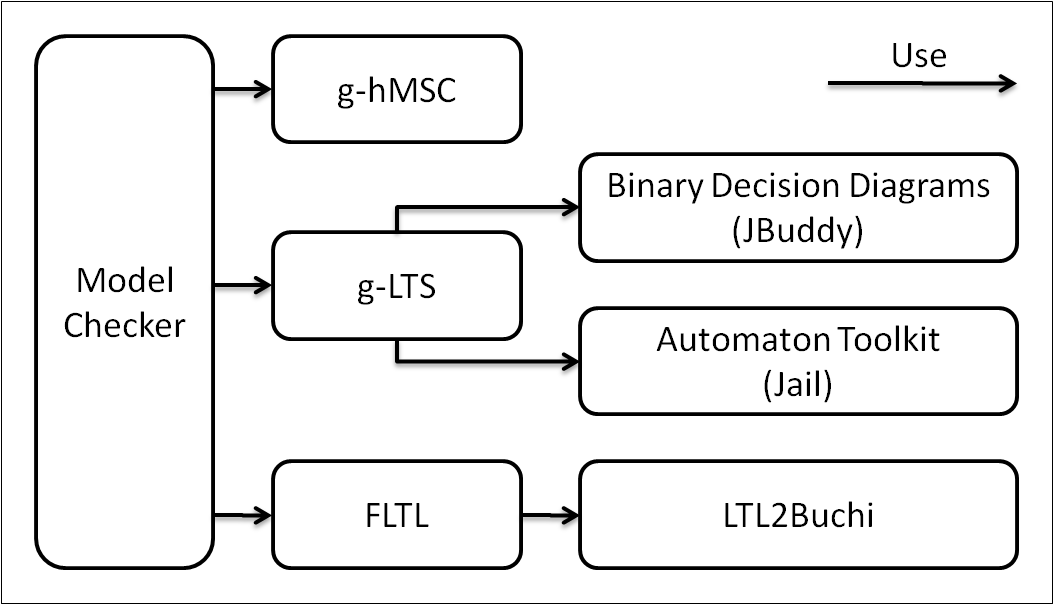
\includegraphics[trim=3mm 3mm 3mm 3mm, clip]{src/7-tool-support/images/model-checker-architecture}}
  \caption{Architecture of the g-hMSC model checker\label{image:model-checker}}
\end{figure}

\begin{description}
\item[Guarded automata] The first module is an implementation of guarded automata. This module reuses our abstract automaton toolkit, namely Jail (which stands for Java Automaton and Induction Library) and a library called JavaBDD\footnote{available at http://javabdd.sourceforge.net/ (last retrieved 2011-08-25)} for efficiently manipulating guards through Binary Decision Diagrams (BDD) \cite{Bryant:1986}.

Jail implements an automaton data structure together with standard algorithms:  minimization, determinization, composition, etc. It has been designed as a fairly abstract library in that it allows states and edges of automata to be decorated with any \emph{(key,value)} pairs. Jail algorithms can be configured to perform specific operations on such decorations when manipulating states and edges. As standard automaton algorithms often compute and/or merge sets of states and edges, Jail provides built-in implementations of aggregation operators (sum, avg, min, max, set union, set intersection, and so on).

A specific configuration of the composition algorithm template in Jail yields the composition operator used on guarded automata. In particular, an aggregation operator for edges relies on BDDs for implementing the conjunction of guards.

\item[FLTL] This second module implements fluents and FLTL temporal properties with the use of the LTL2Buchi\footnote{available at http://ti.arc.nasa.gov/profile/dimitra/projects-tools/ (last retrieved 2011-08-25)} library \cite{Giannakopoulou:2002}. 

LTL2Buchi is used to parse LTL specifications and translates them to B\"uchi automata. Our FLTL module interfaces with LTL2Buchi and translates its B\"uchi automata in our g-LTS. It also translates fluent definitions to g-LTS as explained in Section~\ref{subsection:from-glts-to-lts}.

\item[Guarded hMSC] This structural module implements Guarded hMSC. It mostly consists in the implementation of a graph made of tasks and decision nodes and an API to build them programmatically.
\end{description}

The main module of the model checker provides an API for deriving guarded LTS and LTS from guarded hMSC as well as model-checking them. 
